\chapter{Fundamentação Teórica}\label{cap:fundamentacao}

Este capítulo reúne os fundamentos necessários à compreensão do objeto de estudo. Parte-se dos modelos de linguagem de grande escala e das dificuldades impostas pelo texto clínico, avança-se pela geração aumentada por recuperação e pelos grafos de conhecimento até o GraphRAG, discute-se o comportamento dos modelos diante de contextos longos e encerra-se com os instrumentos de avaliação de classificadores e de anotação de dados, culminando na análise dos trabalhos correlatos e na lacuna que motiva a pesquisa.

\section{Modelos de Linguagem de Grande Escala}\label{sec:llm}

O processamento de linguagem natural passou por transformação profunda com a consolidação dos modelos de linguagem de grande escala (LLMs, do inglês \textit{large language models}), sistemas neurais treinados para estimar a distribuição de probabilidade de sequências textuais e capazes de gerar linguagem coerente a partir de um comando. Esses modelos apoiam-se quase invariavelmente na arquitetura \textit{Transformer}, proposta por \citet{vaswani2017}, cuja inovação central é o mecanismo de autoatenção, que pondera de forma dinâmica a relevância de cada elemento da sequência em relação aos demais, dispensa a recorrência empregada em arquiteturas anteriores e permite o processamento paralelo de sequências longas. A capacidade de modelar dependências de longo alcance e a boa escalabilidade em \textit{hardware} paralelo tornaram essa arquitetura o alicerce sobre o qual modelos com bilhões de parâmetros foram construídos.

O treinamento desses modelos ocorre em duas fases principais. Na primeira, o pré-treinamento auto-supervisionado, o modelo é exposto a grandes volumes de texto não rotulado e otimizado para prever \textit{tokens} a partir de seu contexto, tarefa que não exige anotação humana e que induz a internalização de regularidades sintáticas, semânticas e factuais da língua. O conhecimento assim adquirido fica codificado nos pesos da rede, razão pela qual se fala em conhecimento paramétrico: a informação não é consultada em uma base externa, mas reconstruída pelo próprio modelo no momento da geração.

O modelo pré-treinado, contudo, tende a completar texto de maneira genérica, sem necessariamente atender à intenção expressa em uma instrução. Para corrigir esse comportamento, aplica-se o ajuste por instruções (\textit{instruction tuning}), que refina o modelo sobre pares de instrução e resposta, e técnicas de alinhamento que incorporam preferências humanas, como o aprendizado por reforço a partir de \textit{feedback} humano \citep{ouyang2022}. Esse processo aproxima as respostas do modelo das expectativas do usuário quanto a utilidade, veracidade e adequação.

Ainda assim, o paradigma apresenta limitações estruturais. O conhecimento paramétrico é estático, pois reflete o estado do corpus de treinamento em determinado momento e não incorpora informações posteriores, o que produz defasagem temporal progressiva. A atualização desse conhecimento exige retreinar ou refinar o modelo, operação de custo computacional elevado que não pode ser repetida a cada nova evidência. Em áreas que evoluem com rapidez, como a medicina, essa rigidez compromete a confiabilidade das respostas.

A essas limitações soma-se o fenômeno da alucinação, entendido como a geração de conteúdo fluente e plausível, porém factualmente incorreto ou não sustentado pelas fontes disponíveis \citep{ji2023}. A alucinação decorre da natureza probabilística da geração, de lacunas e ruídos no corpus de treinamento e da ausência de um mecanismo interno de verificação factual, já que o modelo otimiza plausibilidade linguística e não correção. Em contexto clínico, o problema é especialmente grave, pois uma afirmação diagnóstica incorreta apresentada com a mesma fluência de uma correta pode induzir decisões equivocadas, e a checagem por especialista nem sempre é viável em escala.

Dois conceitos operacionais interessam ao restante do trabalho. O primeiro é a tokenização, procedimento que segmenta o texto em unidades sublexicais (\textit{tokens}) antes de submetê-lo ao modelo, de modo que o número de \textit{tokens}, e não o de palavras, passa a ser a unidade de medida do processamento. O segundo é a janela de contexto, o limite máximo de \textit{tokens} que o modelo consegue considerar de uma só vez, somadas entrada e saída. Esse limite condiciona quanto da informação recuperada pode ser fornecido ao modelo em uma única consulta, questão retomada e aprofundada na Seção~\ref{sec:contextos-longos}.

A geração é governada por parâmetros de decodificação, entre os quais a temperatura, que regula a aleatoriedade da amostragem sobre a distribuição de probabilidade dos próximos \textit{tokens}. Valores altos favorecem diversidade; valores próximos de zero aproximam a decodificação de um regime determinístico, em que o \textit{token} mais provável é sempre escolhido. Em pesquisa científica com LLMs, a decodificação determinística é preferível por aumentar a reprodutibilidade dos experimentos, ainda que não a garanta por completo, dado que o paralelismo de \textit{hardware} e as atualizações de modelos acessados por API podem introduzir variação residual.

Fornecer a esses modelos informação externa confiável é, portanto, condição para empregá-los na resposta a perguntas sobre um domínio específico, necessidade que se agrava quando essa informação está registrada em texto clínico não estruturado, objeto da próxima seção.

\section{Prontuários Eletrônicos e o Desafio do Texto Clínico}\label{sec:prontuarios}

O prontuário eletrônico do paciente (PEP; em inglês, \textit{electronic health record}, EHR) é o registro longitudinal e digital das informações de saúde de um indivíduo, mantido por um ou mais serviços assistenciais e destinado a apoiar a continuidade do cuidado, a gestão e a pesquisa. Reúne dados de identificação, história clínica, evolução, prescrições, resultados de exames e desfechos, produzidos por profissionais distintos ao longo do tempo. Parte desse conteúdo é registrada em campos estruturados; parte, em texto livre redigido durante o atendimento.

Os dados clínicos estruturados seguem modelos de representação e vocabulários padronizados que atribuem significado computável a cada item. Padrões de interoperabilidade como o HL7 e sua evolução, o FHIR (\textit{Fast Healthcare Interoperability Resources}), definem como as informações são organizadas e trocadas entre sistemas; terminologias como a Classificação Internacional de Doenças (CID-10) e o SNOMED-CT fornecem códigos unívocos para diagnósticos, procedimentos e achados. Quando presentes, esses elementos permitem consulta direta e agregação confiável. O texto livre, por outro lado, carrega grande parte do raciocínio clínico, como hipóteses, justificativas e nuances de evolução, sem qualquer marcação semântica, e é justamente onde reside a informação necessária para responder perguntas como a que orienta este trabalho.

O texto clínico apresenta características que o tornam particularmente hostil ao processamento automático. Abreviações e siglas são abundantes e não padronizadas, variando entre serviços, especialidades e autores. A ortografia é irregular, com erros de digitação, ausência de acentuação e grafias alternativas. O estilo é telegráfico, com frases nominais, omissão de conectivos e pontuação idiossincrática. A negação e a incerteza são onipresentes, pois se registra com frequência aquilo que foi investigado e afastado, e hipóteses diagnósticas não confirmadas convivem no mesmo documento com diagnósticos estabelecidos, de modo que a simples ocorrência do nome de uma doença não implica que o paciente a tenha. A autoria múltipla acrescenta heterogeneidade de vocabulário e de estrutura ao longo de um mesmo prontuário.

Esses obstáculos são agravados no português clínico brasileiro pela escassez de recursos. Há poucos corpora clínicos anotados e de acesso restrito, não existe vocabulário controlado de referência amplamente adotado equivalente ao que se dispõe em inglês, e a maior parte dos modelos, ontologias e ferramentas de PLN clínico foi desenvolvida para o inglês, o que limita a transferência direta \citep{stammers2025,omar2025}. Traduções de terminologias internacionais nem sempre acompanham o uso efetivo dos profissionais brasileiros.

A variação terminológica configura um problema de normalização de conceitos. Um mesmo achado clínico pode ser expresso por sigla, por sinônimo ou por nomenclatura de época distinta, e todas essas formas precisam ser reconhecidas como referentes à mesma entidade. No domínio hepatológico, a doença hepática gordurosa não alcoólica ilustra bem o fenômeno: as siglas DHGNA e NAFLD, a designação por extenso esteato-hepatite não alcoólica e, mais recentemente, os termos MASLD e MASH, adotados após revisão internacional da nomenclatura \citep{rinella2023}, remetem a condições do mesmo espectro. Um sistema que trate essas formas como conceitos independentes fragmenta a evidência e subestima a presença da doença.

Comparado a outros gêneros textuais especializados, como o jurídico e o científico, o texto clínico é mais adverso para o PLN. Documentos jurídicos e artigos científicos são redigidos para leitura externa, seguem convenções de estrutura e citação, primam pela completude do argumento e passam por revisão editorial. A nota clínica é escrita sob pressão de tempo, como registro para o próprio autor e para colegas que compartilham o contexto do caso, e por isso admite elipse, abreviação e conteúdo implícito. A informação relevante costuma estar dispersa e pressupõe conhecimento que não foi verbalizado no documento.

Extrair uma resposta confiável desse material exige fornecer ao modelo de linguagem trechos pertinentes do próprio prontuário, estratégia que a geração aumentada por recuperação sistematiza e que se descreve a seguir.

\section{Geração Aumentada por Recuperação}\label{sec:rag}

A dependência exclusiva do conhecimento paramétrico restringe o uso de LLMs em domínios especializados ou dinâmicos, tanto pela defasagem quanto pelo risco de alucinação discutidos na Seção~\ref{sec:llm}. A geração aumentada por recuperação (RAG, do inglês \textit{retrieval-augmented generation}), formalizada por \citet{lewis2020}, enfrenta essa limitação ao acoplar ao modelo generativo um componente de recuperação que, dada uma consulta, seleciona trechos pertinentes de uma base externa e os fornece como contexto adicional no momento da geração. O conhecimento passa a ter duas origens, o paramétrico, interno ao modelo, e o não paramétrico, recuperado sob demanda de uma coleção que pode ser atualizada sem retreinamento. A resposta fica ancorada em evidência textual explícita, o que favorece a verificabilidade.

O pipeline canônico do RAG compreende três etapas. Na indexação, realizada uma única vez, os documentos da base são segmentados e convertidos em representações que permitem busca eficiente. Na recuperação, a consulta é comparada a esse índice e os trechos mais relevantes são selecionados. Na geração, esses trechos são concatenados à consulta em um \textit{prompt} e submetidos ao LLM, que produz a resposta final condicionada ao contexto recuperado.

A segmentação dos documentos, ou \textit{chunking}, é decisão de projeto com efeito direto sobre a qualidade do sistema. As estratégias mais simples dividem o texto por número fixo de caracteres ou de \textit{tokens}, com eventual sobreposição entre segmentos vizinhos para não perder informação nas fronteiras. Estratégias semânticas procuram respeitar limites naturais do texto, como parágrafos, seções ou mudanças de tópico. Há um compromisso a administrar, pois segmentos grandes preservam contexto e coerência, mas diluem o sinal relevante e podem esbarrar em limites de \textit{tokens}, ao passo que segmentos pequenos são mais precisos na recuperação, porém correm o risco de fragmentar uma ideia entre unidades distintas. Em texto clínico, telegráfico e pouco estruturado, encontrar esse ponto de equilíbrio é especialmente difícil.

A forma predominante de indexação e recuperação baseia-se em \textit{embeddings}. Cada segmento é mapeado por um modelo codificador para um vetor denso de dimensão fixa, de modo que trechos com significado próximo ocupem posições próximas no espaço vetorial. A consulta é codificada da mesma maneira, e a relevância é estimada por uma medida de proximidade, tipicamente a similaridade de cosseno, que compara a orientação dos vetores independentemente de sua magnitude. Bancos de dados vetoriais armazenam os \textit{embeddings} dos segmentos e implementam busca aproximada por vizinhos mais próximos, o que viabiliza a recuperação em coleções grandes com baixa latência.

Na prática, recupera-se um conjunto dos $k$ segmentos de maior similaridade, valor que equilibra abrangência e custo. Esses segmentos são ordenados e montados no contexto do \textit{prompt}, respeitando o limite da janela discutido anteriormente. A resposta do modelo depende tanto do que foi recuperado quanto da forma como o contexto foi organizado.

O RAG apoiado apenas em similaridade vetorial apresenta limitações reconhecidas. A recuperação seleciona segmentos semanticamente parecidos com a consulta, mas semelhança semântica não equivale a pertinência para responder à pergunta, e informação relevante formulada com outro vocabulário pode ser preterida. O método não modela relações explícitas entre entidades, o que dificulta consultas que exigem encadear vários fatos dispersos em segmentos diferentes, o chamado raciocínio \textit{multi-hop}. Os segmentos mais similares tendem a ser redundantes entre si, o que desperdiça espaço de contexto. Consultas que demandam síntese sobre o conjunto do corpus, e não a localização de uma passagem específica, ficam mal atendidas, pois nenhum segmento isolado contém a resposta \citep{gao2024,edge2024}.

Representar de forma explícita as entidades do corpus e as relações entre elas é uma resposta a essas limitações e conduz aos grafos de conhecimento, tratados na seção seguinte.

\section{Grafos de Conhecimento e Extração de Informação}\label{sec:kg}

Um grafo de conhecimento (KG, do inglês \textit{knowledge graph}) é uma estrutura que representa informação como um conjunto de entidades e das relações que as conectam \citep{hogan2021}. Formalmente, corresponde a um grafo dirigido e rotulado em que os nós denotam entidades do mundo, como pessoas, lugares, doenças ou substâncias, e as arestas denotam relações entre elas. A unidade elementar de informação é a tripla, um par de entidades ligado por um predicado, na forma (sujeito, predicado, objeto), como em (\textit{cirrose}, \textit{causa}, \textit{hipertensão portal}). Um KG é o acúmulo de muitas dessas triplas, o que permite representar redes de fatos interconectados e percorrê-las por meio de consultas estruturadas.

Além das triplas básicas, um KG costuma incorporar enriquecimento semântico e metadados. Entidades e relações podem ser tipadas segundo um esquema ou ontologia, associadas a definições textuais, sinônimos e identificadores externos, e qualificadas por atributos como data ou grau de certeza. Registram-se ainda metadados de proveniência, que indicam a origem de cada afirmação, como o documento e o trecho de onde foi extraída. A proveniência é decisiva em aplicações clínicas, pois permite rastrear uma conclusão até a evidência que a sustenta.

A construção de um KG pode ser manual ou automática. A curadoria manual por especialistas produz grafos precisos e coerentes, mas é lenta, cara e difícil de escalar e de manter atualizada. A construção automática extrai entidades e relações de texto por meios computacionais, com maior cobertura e menor custo, ao preço de introduzir ruído e inconsistências que exigem etapas posteriores de limpeza. Abordagens híbridas combinam extração automática com validação humana seletiva.

A construção automática apoia-se em duas tarefas centrais de extração de informação. O reconhecimento de entidades nomeadas (NER, do inglês \textit{named entity recognition}) identifica no texto as menções a entidades e as classifica em tipos de interesse. A extração de relações (RE, do inglês \textit{relation extraction}) determina quais pares de entidades estão relacionados e sob qual predicado. Historicamente, essas tarefas foram abordadas por sistemas baseados em regras e léxicos, depois por modelos de aprendizado supervisionado treinados sobre corpora anotados e, mais recentemente, por LLMs instruídos a extrair entidades e relações diretamente do texto, com pouca ou nenhuma anotação específica, mediante \textit{prompts} e exemplos. A abordagem por LLM reduz a necessidade de dados rotulados, mas herda os riscos de inconsistência e alucinação já discutidos.

Um mesmo referente costuma aparecer sob formas diferentes ao longo de um corpus, e menções distintas podem designar entidades diferentes apesar de grafias iguais. A resolução de entidades (\textit{entity resolution}) é o processo de decidir quais menções correspondem à mesma entidade, de modo a unificá-las em um único nó. Como comparar todos os pares de menções é inviável em escala, aplicam-se técnicas de bloqueio, que agrupam previamente candidatos plausíveis e restringem a comparação a esses blocos. A decisão final combina similaridade de cadeias de caracteres, similaridade semântica entre \textit{embeddings} das menções e de seus contextos, e desambiguação apoiada na vizinhança no grafo. Sem essa etapa, o grafo fica fragmentado, com a evidência de uma entidade dispersa entre nós duplicados.

No domínio clínico, os nós de interesse correspondem a doenças, sinais e sintomas, medicamentos, exames e procedimentos, e achados laboratoriais, enquanto as arestas capturam relações como uma doença que causa outra, um exame que evidencia um achado ou um fármaco prescrito para uma condição. Um KG assim estruturado, extraído dos prontuários, torna consultável a rede de fatos clínicos de um paciente ou de uma coorte.

Organizar o corpus recuperado como grafo, e não apenas como coleção de segmentos, é o princípio que o GraphRAG incorpora ao pipeline de recuperação, assunto da próxima seção.

\section{GraphRAG}\label{sec:graphrag}

O termo GraphRAG designa, em sentido amplo, a classe de abordagens de geração aumentada por recuperação que empregam um grafo como estrutura intermediária entre o corpus e o modelo generativo, seja para indexar o conteúdo, seja para guiar a recuperação. Sob esse rótulo cabem sistemas com grafos construídos manualmente, grafos derivados de ontologias existentes e grafos extraídos automaticamente do próprio corpus. Em sentido estrito, GraphRAG refere-se com frequência ao sistema homônimo proposto por \citet{edge2024} na Microsoft Research, doravante Microsoft GraphRAG, que extrai o grafo do corpus por meio de um LLM, organiza-o em comunidades hierárquicas e as resume, com o objetivo declarado de responder a consultas de sentido global sobre coleções de documentos, para as quais o RAG vetorial convencional é inadequado. Este trabalho avalia o Microsoft GraphRAG, e as menções a GraphRAG a partir daqui referem-se a essa implementação, salvo indicação em contrário.

O pipeline de indexação do Microsoft GraphRAG encadeia várias etapas, ilustradas na Figura~\ref{fig:graphrag-pipeline}. O corpus é primeiro segmentado em unidades de texto de tamanho controlado. Cada unidade é submetida a um LLM que extrai as entidades presentes, com nome, tipo e uma breve descrição, e as relações entre elas, também descritas em linguagem natural. As menções repetidas de uma mesma entidade ao longo das unidades são deduplicadas e mescladas, e suas descrições são agregadas, o que consolida um grafo único em que nós e arestas acumulam a evidência textual de origem. Sobre esse grafo executa-se um algoritmo de detecção de comunidades, que particiona os nós em grupos densamente conectados. Para cada comunidade, um LLM gera um resumo em linguagem natural a partir das entidades, relações e descrições que ela contém. O produto final da indexação é o conjunto formado pelo grafo, pelas comunidades em seus vários níveis e pelos respectivos resumos, além das unidades de texto originais, tudo disponível para a etapa de consulta.

\begin{figure}[htb]
\centering
\begin{tikzpicture}[
  node distance=6mm and 7mm,
  box/.style={draw, rounded corners, align=center, minimum height=10mm, text width=24mm, font=\footnotesize, fill=gray!8},
  llm/.style={box, fill=gray!22},
  arr/.style={-{Latex[length=2mm]}, thick}
]
\node[box] (corpus) {Corpus de prontuários};
\node[box, right=of corpus] (chunks) {Unidades de texto};
\node[llm, right=of chunks] (extract) {Extração de entidades e relações (LLM)};
\node[box, below=of extract] (merge) {Deduplicação e \textit{merge}};
\node[box, left=of merge] (graph) {Grafo de conhecimento};
\node[box, left=of graph] (comm) {Detecção de comunidades (Leiden)};
\node[llm, below=of comm] (summ) {Resumos de comunidade (LLM)};
\node[box, right=of summ] (index) {Índice: grafo, comunidades e resumos};
\draw[arr] (corpus) -- (chunks);
\draw[arr] (chunks) -- (extract);
\draw[arr] (extract) -- (merge);
\draw[arr] (merge) -- (graph);
\draw[arr] (graph) -- (comm);
\draw[arr] (comm) -- (summ);
\draw[arr] (summ) -- (index);
\end{tikzpicture}
\caption{Pipeline de indexação do Microsoft GraphRAG, do corpus bruto ao índice consultável. Adaptado de \citet{edge2024}.}
\label{fig:graphrag-pipeline}
\end{figure}

A detecção de comunidades no GraphRAG é feita pelo algoritmo de Leiden, proposto por \citet{traag2019} como aprimoramento do método de Louvain. Ambos buscam uma partição do grafo que maximize a modularidade, medida que compara a densidade de arestas dentro das comunidades com a que se esperaria em um grafo aleatório de mesmo grau. O método de Louvain, embora rápido e amplamente usado, pode produzir comunidades internamente mal conectadas, e até desconexas, situação em que um grupo rotulado como comunidade não forma, de fato, um subgrafo coeso. O Leiden acrescenta uma etapa de refinamento que garante que toda comunidade retornada seja internamente conectada, além de convergir para partições de melhor qualidade em menos iterações. O algoritmo é recursivo, no sentido de que, após encontrar uma partição, agrega cada comunidade em um supernó e repete o procedimento sobre o grafo agregado, o que gera uma hierarquia de partições em vez de uma partição única.

Essa recursão produz os níveis de comunidade (\textit{community levels}), níveis de granularidade da partição, ilustrados na Figura~\ref{fig:leiden-hierarquia}. No nível mais agregado, identificado como L0, o grafo é dividido em poucas comunidades amplas, que correspondem a grandes temas do corpus. A cada nível subsequente, as comunidades do nível anterior são subdivididas, de modo que os níveis mais altos contêm muitas comunidades pequenas e tematicamente específicas. Os resumos acompanham essa gradação, pois níveis baixos geram resumos longos e abstratos, que sintetizam grandes porções do corpus, ao passo que níveis altos geram resumos curtos e concretos, próximos do texto de origem. \citet{edge2024} avaliaram condições de nível de comunidade denominadas C0 a C3 e observaram um compromisso, em que os níveis intermediários tendem a favorecer o embasamento factual das respostas, enquanto os níveis mais agregados favorecem a abrangência ao custo de especificidade. Para uma tarefa de classificação diagnóstica, em que a resposta é uma entre poucas categorias e depende de detalhes concretos do prontuário, a especificidade do contexto é prioritária, o que sugere preferência por níveis mais granulares.

\begin{figure}[htb]
\centering
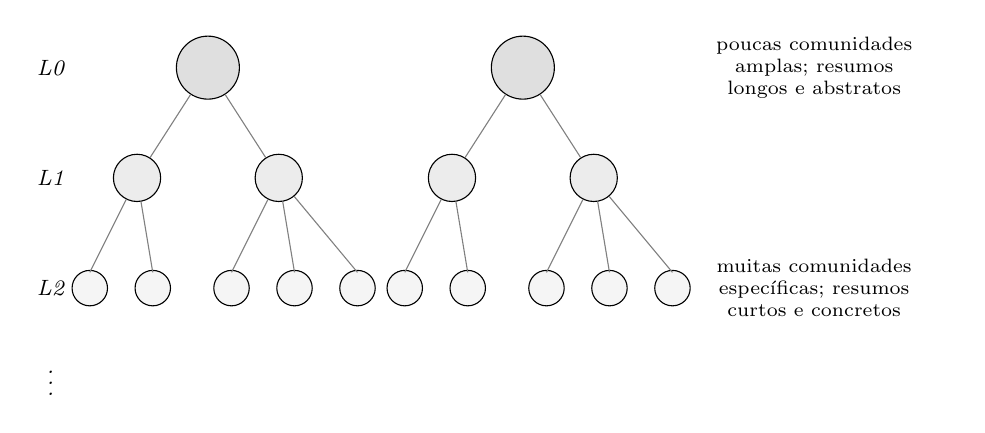
\begin{tikzpicture}[
  lvl/.style={font=\footnotesize\itshape},
  ann/.style={font=\scriptsize, align=center, text width=34mm},
  c0/.style={draw, circle, minimum size=8mm, fill=gray!25, font=\footnotesize},
  c1/.style={draw, circle, minimum size=6mm, fill=gray!15, font=\scriptsize},
  c2/.style={draw, circle, minimum size=4.5mm, fill=gray!8},
  edge/.style={gray}
]
\node[c0] (a) at (0,3) {};
\node[c0] (b) at (4,3) {};
\node[lvl] at (-2,3) {L0};
\node[c1] (a1) at (-0.9,1.6) {};
\node[c1] (a2) at (0.9,1.6) {};
\node[c1] (b1) at (3.1,1.6) {};
\node[c1] (b2) at (4.9,1.6) {};
\node[lvl] at (-2,1.6) {L1};
\foreach \x in {-1.5,-0.7,0.3,1.1,1.9} \node[c2] at (\x,0.2) {};
\foreach \x in {2.5,3.3,4.3,5.1,5.9} \node[c2] at (\x,0.2) {};
\node[lvl] at (-2,0.2) {L2};
\node[lvl] at (-2,-0.9) {$\vdots$};
\node[ann] at (7.7,3) {poucas comunidades amplas; resumos longos e abstratos};
\node[ann] at (7.7,0.2) {muitas comunidades específicas; resumos curtos e concretos};
\draw[edge] (a) -- (a1); \draw[edge] (a) -- (a2);
\draw[edge] (b) -- (b1); \draw[edge] (b) -- (b2);
\draw[edge] (a1) -- (-1.5,0.4); \draw[edge] (a1) -- (-0.7,0.4);
\draw[edge] (a2) -- (0.3,0.4); \draw[edge] (a2) -- (1.1,0.4); \draw[edge] (a2) -- (1.9,0.4);
\draw[edge] (b1) -- (2.5,0.4); \draw[edge] (b1) -- (3.3,0.4);
\draw[edge] (b2) -- (4.3,0.4); \draw[edge] (b2) -- (5.1,0.4); \draw[edge] (b2) -- (5.9,0.4);
\end{tikzpicture}
\caption{Hierarquia de comunidades produzida pela aplicação recursiva do algoritmo de Leiden. Do nível mais agregado (L0) aos mais granulares, cada comunidade é subdividida e os resumos correspondentes tornam-se mais curtos e específicos.}
\label{fig:leiden-hierarquia}
\end{figure}

Na etapa de consulta, o GraphRAG oferece modos de busca distintos, que exploram o índice de maneiras diferentes e estão esquematizados na Figura~\ref{fig:modos-busca}. O modo \textit{basic} recupera diretamente as unidades de texto mais semelhantes à consulta, por similaridade vetorial, sem utilizar a estrutura do grafo, e equivale a um RAG convencional sobre o mesmo corpus. O modo \textit{local} parte da consulta para identificar as entidades mais relevantes no grafo e monta o contexto com essas entidades, sua vizinhança imediata, as relações que as conectam e as unidades de texto associadas, sendo adequado a perguntas centradas em entidades específicas. O modo \textit{global} destina-se a perguntas de sentido global e opera em \textit{map-reduce} sobre os resumos de comunidade de um dado nível, de modo que, na fase de \textit{map}, cada resumo é processado isoladamente para gerar respostas parciais com pontuação de utilidade e, na fase de \textit{reduce}, as respostas parciais mais úteis são combinadas em uma resposta final. O modo \textit{drift} combina as duas orientações em um processo iterativo, que inicia com uma consulta ampla aos resumos de comunidade e, a cada iteração, gera novas subperguntas e as refina com buscas locais, ampliando progressivamente o contexto. O modo \textit{drift} tende a produzir as respostas mais completas, ao custo de um número de chamadas ao LLM substancialmente maior que o dos demais modos.

\begin{figure}[htb]
\centering
\begin{tikzpicture}[
  font=\footnotesize,
  q/.style={draw, rounded corners, fill=gray!15, minimum width=13mm, minimum height=7mm, align=center},
  lbl/.style={font=\footnotesize\itshape},
  ch/.style={draw, fill=gray!5, minimum width=15mm, minimum height=3.6mm},
  ent/.style={draw, circle, fill=gray!15, minimum size=4.5mm, inner sep=0},
  sm/.style={draw, fill=gray!5, minimum width=10mm, minimum height=3.6mm},
  note/.style={align=left, anchor=west, font=\scriptsize, text width=30mm},
  arr/.style={-{Latex[length=1.6mm]}}
]
\node[lbl] at (-3.3,0) {basic};
\node[q] (qb) at (-1.4,0) {consulta};
\node[ch] (b1) at (1.9,0.5) {};
\node[ch] (b2) at (1.9,0.0) {};
\node[ch] (b3) at (1.9,-0.5) {};
\draw[arr] (qb) -- (b2);
\node[note] at (3.1,0) {unidades de texto por similaridade};

\node[lbl] at (-3.3,-2) {local};
\node[q] (ql) at (-1.4,-2) {consulta};
\node[ent] (c) at (1.9,-2) {};
\node[ent] (n1) at (1.0,-1.4) {};
\node[ent] (n2) at (2.8,-1.4) {};
\node[ent] (n3) at (1.0,-2.6) {};
\node[ent] (n4) at (2.8,-2.6) {};
\draw (c)--(n1) (c)--(n2) (c)--(n3) (c)--(n4);
\draw[arr] (ql) -- (c);
\node[note] at (3.6,-2) {entidade central e vizinhança};

\node[lbl] at (-3.3,-4) {global};
\node[q] (qg) at (-1.4,-4) {consulta};
\node[sm] (s1) at (1.5,-3.4) {};
\node[sm] (s2) at (1.5,-4.0) {};
\node[sm] (s3) at (1.5,-4.6) {};
\node[draw, rounded corners, minimum height=6mm] (red) at (3.4,-4) {\textit{reduce}};
\draw[arr] (qg) -- (s1); \draw[arr] (qg) -- (s2); \draw[arr] (qg) -- (s3);
\draw[arr] (s1) -- (red); \draw[arr] (s2) -- (red); \draw[arr] (s3) -- (red);
\node[note] at (4.4,-4) {\textit{map-reduce} sobre resumos de comunidade};

\node[lbl] at (-3.3,-6) {drift};
\node[q] (qd) at (-1.4,-6) {consulta};
\node[sm] (ds) at (1.5,-6) {resumos};
\node[ent] (de) at (3.5,-6) {};
\draw[arr] (qd) -- (ds);
\draw[arr, bend left=30] (ds) to (de);
\draw[arr, bend left=30] (de) to (ds);
\node[note] at (4.4,-6) {iterações global $\leftrightarrow$ local};
\end{tikzpicture}
\caption{Representação esquemática dos quatro modos de busca do Microsoft GraphRAG e da parcela do índice que cada um percorre.}
\label{fig:modos-busca}
\end{figure}

O pipeline padrão do GraphRAG utiliza \textit{prompts} de extração genéricos, concebidos para corpora de domínio aberto, que reconhecem tipos de entidade amplos como pessoa, organização e local. O GraphRAG permite substituir esses \textit{prompts} por versões adaptadas a um domínio, seja por um procedimento automático de ajuste a partir de amostras do corpus, seja por edição manual. A customização define os tipos de entidade pertinentes ao domínio e fornece exemplos \textit{few-shot} alinhados ao vocabulário efetivamente empregado nos documentos. Em hepatologia, isso significa instruir o modelo a extrair entidades como doença hepática, achado laboratorial, exame de imagem e complicação, e ilustrar a extração com trechos representativos de evoluções clínicas, de modo que o grafo resultante reflita as distinções relevantes para a pergunta de pesquisa.

O custo computacional é uma limitação prática incontornável do GraphRAG. A indexação exige uma chamada ao LLM por unidade de texto para a extração e uma chamada por comunidade para a geração de resumos, o que, em um corpus de centenas de documentos com milhares de comunidades, representa um volume elevado de inferências. A consulta também é onerosa, sobretudo nos modos \textit{global} e \textit{drift}, que multiplicam as chamadas ao percorrer resumos ou ao iterar. Esse custo, somado à latência, constitui barreira à adoção e motiva a avaliação criteriosa de quando o ganho de qualidade compensa o esforço adicional. Parte desse ganho, contudo, depende de como o modelo aproveita contextos longos, questão examinada a seguir.
